\documentclass[a4paper, 12pt, english]{article}

% \usepackage[portuges]{babel}
\usepackage[utf8]{inputenc}
\usepackage{amsmath,amssymb}
\usepackage{graphicx}
\usepackage{subfig}
\usepackage[colorinlistoftodos]{todonotes}

\usepackage{indentfirst}
\usepackage{verbatim}
\usepackage{textcomp}
\usepackage{gensymb}
\usepackage{float}
\usepackage{pgfplots}
\pgfplotsset{compat=1.17}

\usepackage{relsize}

\usepackage{lipsum}% http://ctan.org/pkg/lipsum
\usepackage{xcolor}% http://ctan.org/pkg/xcolor
\usepackage{xparse}% http://ctan.org/pkg/xparse
\NewDocumentCommand{\myrule}{O{1pt} O{2pt} O{black}}{%
	\par\nobreak % don't break a page here
	\kern\the\prevdepth % don't take into account the depth of the preceding line
	\kern#2 % space before the rule
	{\color{#3}\hrule height #1 width\hsize} % the rule
	\kern#2 % space after the rule
	\nointerlineskip % no additional space after the rule
}
\usepackage[section]{placeins}

\usepackage{booktabs}
\usepackage{colortbl}%
\newcommand{\myrowcolour}{\rowcolor[gray]{0.925}}

\usepackage[obeyspaces]{url}
\usepackage{etoolbox}
\usepackage[colorlinks,citecolor=black,urlcolor=blue,bookmarks=false,hypertexnames=true]{hyperref}

\usepackage{geometry}
\geometry{
	paper=a4paper, % Change to letterpaper for US letter
	inner=3cm, % Inner margin
	outer=3cm, % Outer margin
	bindingoffset=.5cm, % Binding offset
	top=2cm, % Top margin
	bottom=2cm, % Bottom margin
	%showframe, % Uncomment to show how the type block is set on the page
}
\usepackage{fancyhdr}

% Define header and footer
\pagestyle{fancy}
\fancyhf{}
\lhead{ENER 104L}
\rhead{iSciM, Habib University} % Right-aligned page number in the header
\rfoot{\thepage} % Right footer text
%*******************************************************************************%
%************************************START**************************************%
%*******************************************************************************%
\begin{document}

%************************************TITLE PAGE**************************************%
\begin{titlepage}
	\begin{center}
		\textbf{\LARGE Habib University}\\[0.5cm]
		\textbf{\large iSciM}\\[0.2cm]
		\textbf {\large Fall 2023}\\[0.2cm]
		\vspace{20pt}
		\includegraphics[width=5cm]{../habiblogo.jpg}\\[1cm]
		\par
		\vspace{20pt}
		\textbf{\Large ENER 104L RENEWABLE ENERGY}\\
		\vspace{15pt}
		\myrule[1pt][7pt]
		\textbf{\LARGE  LABORATORY REPORT 7}\\
		\vspace{15pt}
		\textbf{\large Heat Energy from Solar Energy}\\
		\myrule[1pt][7pt]
		\vspace{25pt}
		\begin{tabular}{@{}p{5cm}p{3cm}@{}}
			\textbf{\large Student Name} & \textbf{\large Student ID} \\
			Ali Asghar Yousuf            & ay06993                    \\ % No1 
			Syed Ibrahim Ali Haider      & sh06565                    \\ % No2
		\end{tabular}

		\vspace{10pt}
		\begin{tabular}{@{}p{5cm}p{3cm}@{}}
			\textbf{\large Group Name} & \textbf{\large Group No.} \\
			Insane Fr                  & 1                         \\
		\end{tabular}

		\vspace{45pt}
		\textbf {\large Lab Instructors:}\\[0.2cm]
		\Large {Paishwa Naqvi}\\[0.1cm]
		\Large {Mah Noor Jamil}\\[0.1cm]
		\Large {Amber Talat}\\[0.1cm]
	\end{center}

	\par
	\vfill
	\begin{center}
		\textbf{\today}\\
	\end{center}

\end{titlepage}

%************************************TABLE OF CONTENTS**************************************%

%  %Sumário
%  \newpage
%  \tableofcontents
%  \thispagestyle{empty}
%  %End Sumário

%********************************%
%***********SECTION 1************%
%********************************%
\newpage
\section{Objectives}
\begin{itemize}
	\item To understand the concept of solar energy and its conversion to heat energy.
	\item To understand how the color of an object affects the amount of heat energy it
	      absorbs.
	\item To understand the role of insulation in reducing heat loss.
	\item To understand the principle of the greenhouse effect.
\end{itemize}

\section{Abstract}
The objective of this lab was to understand the concept of solar energy and its
conversion to heat energy and why white tents are used in deserts. The
experiment was divided into three parts. In the first part, we observed the
effect of color on the amount of heat energy absorbed by an object. In the
second part, we observed the effect of insulation on the amount of heat energy
absorbed by an object. In the third part, we observed the effect of the
greenhouse effect on the amount of heat energy abosrbed and then retained by an
object.

\section{Result and Analysis}
\subsection{Part A}
$T_i$ represents the initial temperature of the plate and $T_f$ represents the
final temperature of the plate.
\begin{table}[H]
	\centering
	\caption{Temperature Table for Part A}
	\label{tab:table1}
	\begin{tabular}{@{}llll@{}}
		\toprule
		            & \textbf{$T_i$ (\degree C)} & \textbf{$T_f$ (\degree C)} & \textbf{$\Delta T$ (\degree C)} \\ \midrule
		White Plate & 21                         & 24                         & 3                               \\
		Black Plate & 22                         & 30                         & 8                               \\ \bottomrule
	\end{tabular}
\end{table}

The temperature of the white plate increased by 3\degree C while the
temperature of the black plate increased by 8\degree C. This is because the
white plate reflects most of the light falling on it while the black plate
absorbs most of the light falling on it. Therefore the temperature increase of
the black plate was higher than that of the white plate.
\subsection{Part B}
\begin{table}[H]
	\centering
	\caption{Temperature Table for Part B}
	\label{tab:table2}
	\begin{tabular}{@{}llll@{}}
		\toprule
		          & \textbf{$T_i$ (\degree C)} & \textbf{$T_f$ (\degree C)} & \textbf{$\Delta T$ (\degree C)} \\ \midrule
		Uncovered & 22                         & 30                         & 8                               \\
		Insulated & 23                         & 38                         & 15                              \\ \bottomrule
	\end{tabular}
\end{table}

The temperature of the uncovered plate increased by 8\degree C while the
temperature of the insulated plate increased by 15\degree C. This is because
the heat loss from the insulated plate was less than that of the uncovered
plate. Therefore the temperature increase of the insulated plate was
significantly higher than that of the uncovered plate.

\subsection{Part C}
$T_0$ represents the temperature of the plate without the plexiglass and $T_p$
represents the temperature of the plate with the plexiglass.
\begin{table}[H]
	\centering
	\caption{Temperature Table for Part C}
	\label{tab:table3}
	\begin{tabular}{@{}lll@{}}
		\toprule
		\textbf{Time (min)} & \textbf{$T_0$ (\degree C)} & \textbf{$T_p$ (\degree C)} \\ \midrule
		0                   & 22                         & 22                         \\
		1                   & 26                         & 27                         \\
		2                   & 30                         & 31                         \\
		3                   & 34                         & 35                         \\
		4                   & 38                         & 39                         \\
		5                   & 41                         & 42                         \\
		6                   & 43                         & 45                         \\
		7                   & 45                         & 47                         \\
		\bottomrule \multicolumn{3}{l}{Lamp turned off}                               \\ \bottomrule
		8                   & 45                         & 47                         \\
		9                   & 43                         & 46                         \\
		10                  & 41                         & 44                         \\
		11                  & 39                         & 43                         \\
		12                  & 38                         & 42                         \\
		13                  & 37                         & 41                         \\
		14                  & 35                         & 40                         \\
		15                  & 34                         & 39                         \\
		\bottomrule
	\end{tabular}
\end{table}

The temperature of the plate without the plexiglass increased by 23\degree C
while the temperature of the plate with the plexiglass increased by 25\degree C
over 7 mins when the lamp was turned on. Similarly, after the lamp was turned
off, the temperature of the plate without the plexiglass decreased by 11\degree
C while the temperature of the plate with the plexiglass decreased by 8\degree
C.

This is because the plexiglass creates a greenhouse effect and reduces the heat
loss from the plate. Therefore the temperature increase of the plate with the
plexiglass was higher than that of the plate without the plexiglass when the
lamp was turned on and the temperature decrease of the plate with the
plexiglass was lower than that of the plate without the plexiglass when the
lamp was turned off.

% plot the above table as a graph in latex
\begin{figure}[H]
\centering
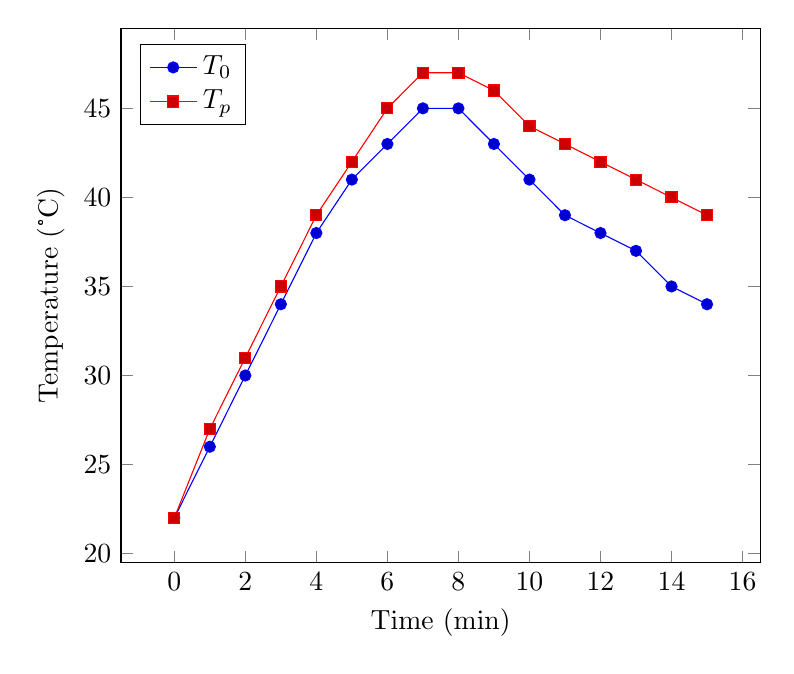
\begin{tikzpicture}
\begin{axis}[
		width=0.8\textwidth,
		xlabel=Time (min),
		ylabel=Temperature (\degree C),
		legend pos=north west,
		legend cell align={left},
		% enlarge x limits=0.15,
	]

	\addplot table[x expr=\coordindex, y=T0] {
			Time T0 Tp
			0    22 22
			1    26 27
			2    30 31
			3    34 35
			4    38 39
			5    41 42
			6    43 45
			7    45 47
			8    45 47
			9    43 46
			10   41 44
			11   39 43
			12   38 42
			13   37 41
			14   35 40
			15   34 39
		};
	\addlegendentry{$T_0$}

	\addplot table[x expr=\coordindex, y=Tp] {
			Time T0 Tp
			0    22 22
			1    26 27
			2    30 31
			3    34 35
			4    38 39
			5    41 42
			6    43 45
			7    45 47
			8    45 47
			9    43 46
			10   41 44
			11   39 43
			12   38 42
			13   37 41
			14   35 40
			15   34 39
		};
	\addlegendentry{$T_p$}
\end{axis}
\end{tikzpicture}
\caption{Temperature Graph for Part C}
\end{figure}

\section{Conclusion}
The results of the experiment showed that the color of an object affects the
amount of heat energy it absorbs, darker colors absorb more light than lighter
colors which results in higher energy absorption. The results also showed that
insulation reduces heat loss and therefore increases the amount of heat energy
absorbed by an object. Finally, we learnt that the greenhouse effect increases
the amount of heat energy absorbed and then retained by an object.

\end{document}